
%% bare_conf.tex
%% V1.3
%% 2007/01/11
%% by Michael Shell
%% See:
%% http://www.michaelshell.org/
%% for current contact information.
%%
%% This is a skeleton file demonstrating the use of IEEEtran.cls
%% (requires IEEEtran.cls version 1.7 or later) with an IEEE conference paper.
%%
%% Support sites:
%% http://www.michaelshell.org/tex/ieeetran/
%% http://www.ctan.org/tex-archive/macros/latex/contrib/IEEEtran/
%% and
%% http://www.ieee.org/

%%*************************************************************************
%% Legal Notice:
%% This code is offered as-is without any warranty either expressed or
%% implied; without even the implied warranty of MERCHANTABILITY or
%% FITNESS FOR A PARTICULAR PURPOSE!
%% User assumes all risk.
%% In no event shall IEEE or any contributor to this code be liable for
%% any damages or losses, including, but not limited to, incidental,
%% consequential, or any other damages, resulting from the use or misuse
%% of any information contained here.
%%
%% All comments are the opinions of their respective authors and are not
%% necessarily endorsed by the IEEE.
%%
%% This work is distributed under the LaTeX Project Public License (LPPL)
%% ( http://www.latex-project.org/ ) version 1.3, and may be freely used,
%% distributed and modified. A copy of the LPPL, version 1.3, is included
%% in the base LaTeX documentation of all distributions of LaTeX released
%% 2003/12/01 or later.
%% Retain all contribution notices and credits.
%% ** Modified files should be clearly indicated as such, including  **
%% ** renaming them and changing author support contact information. **
%%
%% File list of work: IEEEtran.cls, IEEEtran_HOWTO.pdf, bare_adv.tex,
%%                    bare_conf.tex, bare_jrnl.tex, bare_jrnl_compsoc.tex
%%*************************************************************************

% *** Authors should verify (and, if needed, correct) their LaTeX system  ***
% *** with the testflow diagnostic prior to trusting their LaTeX platform ***
% *** with production work. IEEE's font choices can trigger bugs that do  ***
% *** not appear when using other class files.                            ***
% The testflow support page is at:
% http://www.michaelshell.org/tex/testflow/



% Note that the a4paper option is mainly intended so that authors in
% countries using A4 can easily print to A4 and see how their papers will
% look in print - the typesetting of the document will not typically be
% affected with changes in paper size (but the bottom and side margins will).
% Use the testflow package mentioned above to verify correct handling of
% both paper sizes by the user's LaTeX system.
%
% Also note that the "draftcls" or "draftclsnofoot", not "draft", option
% should be used if it is desired that the figures are to be displayed in
% draft mode.
%
\documentclass[conference, 10pt]{IEEEtran}
% Add the compsoc option for Computer Society conferences.
%
% If IEEEtran.cls has not been installed into the LaTeX system files,
% manually specify the path to it like:
% \documentclass[conference]{../sty/IEEEtran}





% Some very useful LaTeX packages include:
% (uncomment the ones you want to load)


% *** MISC UTILITY PACKAGES ***
%
%\usepackage{ifpdf}
% Heiko Oberdiek's ifpdf.sty is very useful if you need conditional
% compilation based on whether the output is pdf or dvi.
% usage:
% \ifpdf
%   % pdf code
% \else
%   % dvi code
% \fi
% The latest version of ifpdf.sty can be obtained from:
% http://www.ctan.org/tex-archive/macros/latex/contrib/oberdiek/
% Also, note that IEEEtran.cls V1.7 and later provides a builtin
% \ifCLASSINFOpdf conditional that works the same way.
% When switching from latex to pdflatex and vice-versa, the compiler may
% have to be run twice to clear warning/error messages.






% *** CITATION PACKAGES ***
%
%\usepackage{cite}
% cite.sty was written by Donald Arseneau
% V1.6 and later of IEEEtran pre-defines the format of the cite.sty package
% \cite{} output to follow that of IEEE. Loading the cite package will
% result in citation numbers being automatically sorted and properly
% "compressed/ranged". e.g., [1], [9], [2], [7], [5], [6] without using
% cite.sty will become [1], [2], [5]--[7], [9] using cite.sty. cite.sty's
% \cite will automatically add leading space, if needed. Use cite.sty's
% noadjust option (cite.sty V3.8 and later) if you want to turn this off.
% cite.sty is already installed on most LaTeX systems. Be sure and use
% version 4.0 (2003-05-27) and later if using hyperref.sty. cite.sty does
% not currently provide for hyperlinked citations.
% The latest version can be obtained at:
% http://www.ctan.org/tex-archive/macros/latex/contrib/cite/
% The documentation is contained in the cite.sty file itself.






% *** GRAPHICS RELATED PACKAGES ***
%
\ifCLASSINFOpdf
  % \usepackage[pdftex]{graphicx}
  % declare the path(s) where your graphic files are
  % \graphicspath{{../pdf/}{../jpeg/}}
  % and their extensions so you won't have to specify these with
  % every instance of \includegraphics
  % \DeclareGraphicsExtensions{.pdf,.jpeg,.png}
\else
  % or other class option (dvipsone, dvipdf, if not using dvips). graphicx
  % will default to the driver specified in the system graphics.cfg if no
  % driver is specified.
  % \usepackage[dvips]{graphicx}
  % declare the path(s) where your graphic files are
  % \graphicspath{{../eps/}}
  % and their extensions so you won't have to specify these with
  % every instance of \includegraphics
  % \DeclareGraphicsExtensions{.eps}
\fi
% graphicx was written by David Carlisle and Sebastian Rahtz. It is
% required if you want graphics, photos, etc. graphicx.sty is already
% installed on most LaTeX systems. The latest version and documentation can
% be obtained at:
% http://www.ctan.org/tex-archive/macros/latex/required/graphics/
% Another good source of documentation is "Using Imported Graphics in
% LaTeX2e" by Keith Reckdahl which can be found as epslatex.ps or
% epslatex.pdf at: http://www.ctan.org/tex-archive/info/
%
% latex, and pdflatex in dvi mode, support graphics in encapsulated
% postscript (.eps) format. pdflatex in pdf mode supports graphics
% in .pdf, .jpeg, .png and .mps (metapost) formats. Users should ensure
% that all non-photo figures use a vector format (.eps, .pdf, .mps) and
% not a bitmapped formats (.jpeg, .png). IEEE frowns on bitmapped formats
% which can result in "jaggedy"/blurry rendering of lines and letters as
% well as large increases in file sizes.
%
% You can find documentation about the pdfTeX application at:
% http://www.tug.org/applications/pdftex





% *** MATH PACKAGES ***
%
%\usepackage[cmex10]{amsmath}
% A popular package from the American Mathematical Society that provides
% many useful and powerful commands for dealing with mathematics. If using
% it, be sure to load this package with the cmex10 option to ensure that
% only type 1 fonts will utilized at all point sizes. Without this option,
% it is possible that some math symbols, particularly those within
% footnotes, will be rendered in bitmap form which will result in a
% document that can not be IEEE Xplore compliant!
%
% Also, note that the amsmath package sets \interdisplaylinepenalty to 10000
% thus preventing page breaks from occurring within multiline equations. Use:
%\interdisplaylinepenalty=2500
% after loading amsmath to restore such page breaks as IEEEtran.cls normally
% does. amsmath.sty is already installed on most LaTeX systems. The latest
% version and documentation can be obtained at:
% http://www.ctan.org/tex-archive/macros/latex/required/amslatex/math/





% *** SPECIALIZED LIST PACKAGES ***
%
%\usepackage{algorithmic}
% algorithmic.sty was written by Peter Williams and Rogerio Brito.
% This package provides an algorithmic environment fo describing algorithms.
% You can use the algorithmic environment in-text or within a figure
% environment to provide for a floating algorithm. Do NOT use the algorithm
% floating environment provided by algorithm.sty (by the same authors) or
% algorithm2e.sty (by Christophe Fiorio) as IEEE does not use dedicated
% algorithm float types and packages that provide these will not provide
% correct IEEE style captions. The latest version and documentation of
% algorithmic.sty can be obtained at:
% http://www.ctan.org/tex-archive/macros/latex/contrib/algorithms/
% There is also a support site at:
% http://algorithms.berlios.de/index.html
% Also of interest may be the (relatively newer and more customizable)
% algorithmicx.sty package by Szasz Janos:
% http://www.ctan.org/tex-archive/macros/latex/contrib/algorithmicx/




% *** ALIGNMENT PACKAGES ***
%
%\usepackage{array}
% Frank Mittelbach's and David Carlisle's array.sty patches and improves
% the standard LaTeX2e array and tabular environments to provide better
% appearance and additional user controls. As the default LaTeX2e table
% generation code is lacking to the point of almost being broken with
% respect to the quality of the end results, all users are strongly
% advised to use an enhanced (at the very least that provided by array.sty)
% set of table tools. array.sty is already installed on most systems. The
% latest version and documentation can be obtained at:
% http://www.ctan.org/tex-archive/macros/latex/required/tools/


%\usepackage{mdwmath}
%\usepackage{mdwtab}
% Also highly recommended is Mark Wooding's extremely powerful MDW tools,
% especially mdwmath.sty and mdwtab.sty which are used to format equations
% and tables, respectively. The MDWtools set is already installed on most
% LaTeX systems. The lastest version and documentation is available at:
% http://www.ctan.org/tex-archive/macros/latex/contrib/mdwtools/


% IEEEtran contains the IEEEeqnarray family of commands that can be used to
% generate multiline equations as well as matrices, tables, etc., of high
% quality.


%\usepackage{eqparbox}
% Also of notable interest is Scott Pakin's eqparbox package for creating
% (automatically sized) equal width boxes - aka "natural width parboxes".
% Available at:
% http://www.ctan.org/tex-archive/macros/latex/contrib/eqparbox/





% *** SUBFIGURE PACKAGES ***
%\usepackage[tight,footnotesize]{subfigure}
% subfigure.sty was written by Steven Douglas Cochran. This package makes it
% easy to put subfigures in your figures. e.g., "Figure 1a and 1b". For IEEE
% work, it is a good idea to load it with the tight package option to reduce
% the amount of white space around the subfigures. subfigure.sty is already
% installed on most LaTeX systems. The latest version and documentation can
% be obtained at:
% http://www.ctan.org/tex-archive/obsolete/macros/latex/contrib/subfigure/
% subfigure.sty has been superceeded by subfig.sty.



%\usepackage[caption=false]{caption}
%\usepackage[font=footnotesize]{subfig}
% subfig.sty, also written by Steven Douglas Cochran, is the modern
% replacement for subfigure.sty. However, subfig.sty requires and
% automatically loads Axel Sommerfeldt's caption.sty which will override
% IEEEtran.cls handling of captions and this will result in nonIEEE style
% figure/table captions. To prevent this problem, be sure and preload
% caption.sty with its "caption=false" package option. This is will preserve
% IEEEtran.cls handing of captions. Version 1.3 (2005/06/28) and later
% (recommended due to many improvements over 1.2) of subfig.sty supports
% the caption=false option directly:
%\usepackage[caption=false,font=footnotesize]{subfig}
%
% The latest version and documentation can be obtained at:
% http://www.ctan.org/tex-archive/macros/latex/contrib/subfig/
% The latest version and documentation of caption.sty can be obtained at:
% http://www.ctan.org/tex-archive/macros/latex/contrib/caption/




% *** FLOAT PACKAGES ***
%
%\usepackage{fixltx2e}
% fixltx2e, the successor to the earlier fix2col.sty, was written by
% Frank Mittelbach and David Carlisle. This package corrects a few problems
% in the LaTeX2e kernel, the most notable of which is that in current
% LaTeX2e releases, the ordering of single and double column floats is not
% guaranteed to be preserved. Thus, an unpatched LaTeX2e can allow a
% single column figure to be placed prior to an earlier double column
% figure. The latest version and documentation can be found at:
% http://www.ctan.org/tex-archive/macros/latex/base/



%\usepackage{stfloats}
% stfloats.sty was written by Sigitas Tolusis. This package gives LaTeX2e
% the ability to do double column floats at the bottom of the page as well
% as the top. (e.g., "\begin{figure*}[!b]" is not normally possible in
% LaTeX2e). It also provides a command:
%\fnbelowfloat
% to enable the placement of footnotes below bottom floats (the standard
% LaTeX2e kernel puts them above bottom floats). This is an invasive package
% which rewrites many portions of the LaTeX2e float routines. It may not work
% with other packages that modify the LaTeX2e float routines. The latest
% version and documentation can be obtained at:
% http://www.ctan.org/tex-archive/macros/latex/contrib/sttools/
% Documentation is contained in the stfloats.sty comments as well as in the
% presfull.pdf file. Do not use the stfloats baselinefloat ability as IEEE
% does not allow \baselineskip to stretch. Authors submitting work to the
% IEEE should note that IEEE rarely uses double column equations and
% that authors should try to avoid such use. Do not be tempted to use the
% cuted.sty or midfloat.sty packages (also by Sigitas Tolusis) as IEEE does
% not format its papers in such ways.

\usepackage{graphicx}
\usepackage{color}
\usepackage{placeins}
\usepackage{float}
\usepackage{tabularx,colortbl}
\usepackage{algpseudocode}
\usepackage{algorithm}
\usepackage{qtree}
\usepackage{url}
\usepackage{pgfplots}

\begin{document}
%
% paper title
% can use linebreaks \\ within to get better formatting as desired
\title{Spatial Clustering Algorithms: A Selective Survey}


% author names and affiliations
% use a multiple column layout for up to three different
% affiliations
\author{\IEEEauthorblockN{Baskin, Sean \\
                          Reinsmidt, Eric \\
                          Sidella, Pallavi}
\IEEEauthorblockA{Department of Engineering and Computer Science\\
University of Tennessee at Chattanooga\\
Chattanooga, Tennessee, U.S.A.\\}}

% make the title area
\maketitle


\begin{abstract}
%\boldmath
% Please include a brief abstract here. The abstract should be limited to 50-200 words and should concisely state what was done, how it was done, principal results, and their significance.
Our primary motivation for undertaking this study is to test the reliability of an algorithm's theoretically estimated running time and the experimental results that follow. Secondary considerations are pursuing algorithms that operate on relevant themes emerging in computer science such as massive datasets. The following algorithms will be implemented and evaluated:
\vspace{1 mm}
\begin{itemize}
  \item BIRCH
  \item DBSCAN
  \item Fuzzy K-Means
\end{itemize}
\vspace{1 mm}
Our research involves determining which of the selected algorithms provides the most efficient estimated runtime and most efficient experimental runtime in a real-world implementation with regard to spatial-specific metrics including:
\vspace{1 mm}
\begin{itemize}
  \item The ability to handle dimensionality
  \item Handle irregularly shaped clusters
  \item Insensitivity to noise
  \item Independence of the data input order
\end{itemize}
\vspace{1 mm}

\end{abstract}

\section{Introduction}
Due to advances in scientific data collection, we now have large and continuously growing amounts of data. Clustering is one of the techniques used in data mining and is also a common technique in statistical data analysis and spatial data mining. Spatial data consists of geometric information which can be continuous or discrete. Spatial clustering can be applied on spatial data sets for successful data mining. Even though there are number of different methods proposed for spatial clustering, they can be divided into three types which are partition-based clustering, hierarchical clustering and density-based clustering.  As the name suggests, partition based clustering partitions the data into groups of similar objects in a cluster compared to the objects in other clusters.  K-means, K-medoids and Fuzzy C means are few of the popular partition-based clustering algorithms.  Hierarchical clustering is based on the idea of building a tree of data that can merge similar groups of points together by performing a sequence of partitions. BIRCH, CHAMELEON, and CURE are some of the examples of hierarchical clustering.  Density based clustering is based on grouping of clusters as areas of higher density than the remaining data. DBSCAN, GDBSCAN and OPTICS are some of the examples of density based clustering. Out of each the three general types of spatial clustering algorithms, we have chosen one algorithm to run performance testing.

%==================================
% BIRCH ALGORITHM
%==================================
\subsection{BIRCH}

The Balanced Iterative Reducing and Clustering using Hierarchies (BIRCH) algorithm was conceived of as a way to balance the need to cluster extremely large datasets in situations where time and memory are limited. To achieve the time requirement, BIRCH only scans a dataset one time, which improves the rumtime efficiency. While it may be counterintuitive that it only scans a dataset one time while also having a memory restricted system, BIRCH accomplishes this by building a Clustering Feature Tree (CF Tree) that can cluster data in chunks as it is scanned piecemeal \cite{birch}.

The BIRCH algorithm consists of four phases, two of which are optional:
\vspace{1 mm}
\begin{enumerate}
  \item Creation of the CF Tree scanned into memory in $O(n)$
  \item Resizing tree to remove outliers (optional)
  \item Clustering using custom hierarchichal agglomerative clustering algorithm in $O(n^2)$
  \item Additional scanning of the data for improved outlier removal (optional)
\end{enumerate}
\vspace{1 mm}

\begin{algorithm}
\caption{BIRCH}
\begin{algorithmic}[1]
\Procedure{Birch}{$add, inputs, here$}
\EndProcedure
\end{algorithmic}
\end{algorithm}

\begin{center}
\includegraphics[width=90mm]{cf_tree.png}\end{center}

%==================================% 
% DBSCAN ALGORITHM
%==================================
\subsection{DBSCAN}
Intro about DBSCAN here, blah, blah, blah

\begin{algorithm}
\caption{DBSCAN}
\begin{algorithmic}[1]
\Procedure{Dbscan}{$D, \epsilon,MinPts$}\Comment{$D$ set of points is unclassified}
  \State $clusterID = 0$
  \For{$i\gets 1, n$}
      \State $p \gets D[i]$
      \State $p.visited \gets true$    \Comment{Mark $p$ as visited}
      \If{$p.clusterID = UNCLASSIFIED$}
        \If {\Call{ExpandCluster}{{$D, p, clusterID, \epsilon, MinPts$}}}
          \State $clusterID \gets nextID(clusterID)$
        \EndIf
      \EndIf
  \EndFor
\EndProcedure
\Statex
\Procedure{ExpandCluster}{}
\EndProcedure
\end{algorithmic}
\end{algorithm}

%==================================
% FUZZY K-MEANS ALGORITHM
%==================================
\subsection{Fuzzy K-Means}
Fuzzy K-Means clustering (FKM) algorithm is an unsupervised clustering algorithm which can be
applied to wide range of applications like medical imaging, agricultural engineering, astronomy,
geology, shape analysis, chemistry and many more applications \cite{pattern}. FKM performs iteratively the partition step until convergence. Extensive computations which are usually required to generate cluster representatives can be accomplished through the iteration process. FKM algorithm partitions data points into $k$ clusters

\begin{algorithm}
\caption{Fuzzy K-Means}
\begin{algorithmic}[1]
\State Input: $D$ (training set with n points), $K$ (number of clusters), $f$ (fuzzy coefficient), $m$ (max\_iterations)
\State Output: Converged points
\Procedure{Fuzzy K-Means}{$D, K, f, m$}
  \State Initialize membership values $V[0,1]$ for $K$ clusters
  \State $Max=Max+1$
  \For{$||V-V1|| <= \epsilon$ OR $Max=m$}
    \For{$i\gets 1, K$}
        \State Calculate centroids $C$
        \State Calculate new distance of $n$ to centric
        \State $V1 = V$
        \State Update $V$ with new membership
    \EndFor
  \EndFor
\EndProcedure
\Statex
\Procedure{ExpandCluster}{}
\EndProcedure
\end{algorithmic}
\end{algorithm}

%==================================
% END OF INTRODUCTION
%==================================

\section{Asymptotic Evaluation}

\subsection{BIRCH}
\subsection{DBSCAN}
\subsection{Fuzzy K-Means}
The asymptotic efficiency of FKM algorithm has the following notations:\\*
$i$ number of iterations over the entire dataset\\*
$n$ number of data points in the data set\\*
$c$ number of clusters\\*
$d$ number of dimension in the data set\\*

Hence the time complexity of FKM algorithm is $O(ndc^2i$), where growth of $i$ is slower than $n, c, and\:d$.

The space complexity of FKM algorithm is $O(nd+nc$), where $nd$ is the size of the data set with $d$ dimensions; and $nc$ is the size of the initial membership matrix.

For large data sets, which cannot be fully loaded into the memory, FKM algorithm will access
disk for every iteration, thus increasing the input/output complexity $O(ndi)$.

\begin{equation}
\alpha+\beta=\chi
\end{equation}

\section{Empirical Evaluation}
TALK ABOUT OUR TESTING METHOD HERE

\subsection{Testing Environment}
\begin{center}
Intel Core i7 @ 2.3GHz per core\\*
16GB DDR3 @ 1600MHz
\end{center}

\subsection{Results}

\begin{table}[h]
\begin{center}
\caption{Comparison of Algorithm runtimes, in seconds} \label{Table1Label}
\begin{tabular}{|c|c|c|c|}
 \hline
 Number of data points & BIRCH & DBSCAN& Fuzzy K-means \\
 \hline
 150,000 & 25.030436 & 75 & 155.195909\\
 \hline
 75,000 & 11.624714 & 45 & 74.441829\\
 \hline
 37,500 & 5.232216 & 25 & 38.501281\\
 \hline
 18,750 & 2.363530 & 10 & 19.471102\\
 \hline
 9375 & 1.031360 & 5 & 9.723024\\
 \hline
 4688 & 0.447284 & 2 & 4.771375\\
 \hline
 2344 & 0.203005 & 1 & 2.414930\\
 \hline
 1172 & 0.091562 & 0.5 & 1.214021\\
 \hline
 586 & 0.043213 & 0.25 & 0.640441\\
 \hline
 297 & 0.020289 & 0.125 & 0.338978\\
 \hline
\end{tabular}
\end{center}
\end{table}

% (150000,155.195909)
% (75000,74.441829)
% (37500,38.501281)
% (18750,19.471102)
% (9375,9.723024)
% (4688,4.771375)
% (2344,2.414930)
% (1172,1.214021)
% (586,0.640441)
% (297,0.338978)


\begin{center}
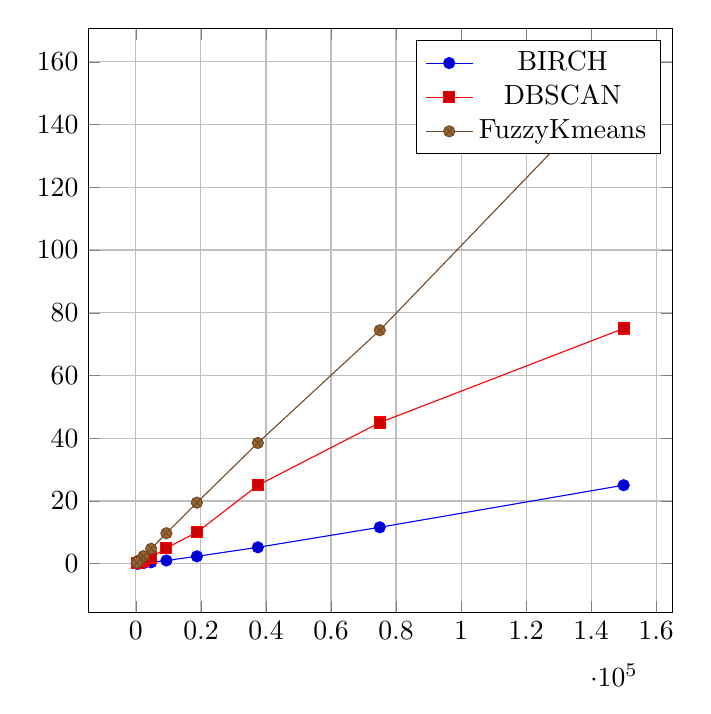
\begin{tikzpicture}
\begin{axis}[
    height=9cm,
    width=9cm,
    grid=major,
  ]
  \addplot coordinates {
    (150000,25.030436)
    (75000,11.624714)
    (37500,5.232216)
    (18750,2.363530)
    (9375,1.031360)
    (4688,0.447284)
    (2344,0.203005)
    (1172,0.091562)
    (586,0.043213)
    (297,0.020289)
  };
  \addlegendentry{BIRCH}
  \addplot coordinates {
    (150000,75)
    (75000,45)
    (37500,25)
    (18750,10)
    (9375,5)
    (4688,2)
    (2344,1)
    (1172,0.5)
    (586,0.25)
    (297,0.125)
  };
  \addlegendentry{DBSCAN}
  \addplot coordinates {
    (150000,155.195909)
    (75000,74.441829)
    (37500,38.501281)
    (18750,19.471102)
    (9375,9.723024)
    (4688,4.771375)
    (2344,2.414930)
    (1172,1.214021)
    (586,0.640441)
    (297,0.338978)
  };
  \addlegendentry{FuzzyKmeans}
\end{axis}
\end{tikzpicture}
\end{center}

\section{Discussion and Conclusion}
Stuff here about what we learned, etc.

\begin{thebibliography}{1}

\bibitem{survey} R. Xu, D. Wunsch, ``Survey of Clustering Algorithms'', \emph{IEEE Transactions on Neural Networks}, vol. 16, no. 3, May, 2005, available at 
\url{http://axon.cs.byu.edu/Dan/678/papers/Cluster/Xu.pdf}.

\bibitem{database} Chandra E., Anuradha V.P. ``A Survey on Clustering Algorithms for Data in Spatial Database Management Systems'', \emph{International Journal of Computer Applications}, available at
\url{http://www.ijcaonline.org/volume24/number9/pxc3873975.pdf}

\bibitem{categorization} N. Soni, A. Ganatra, ``Categorization of Several Clustering Algorithms from Different Perspective: A Review'', \emph{International Journal of Advanced Research in Computer Science and Software Engineering}, vol. 2, iss. 8, August, 2012, available at
\url{http://www.ijarcsse.com/docs/papers/8_August2012/Volume_2_issue_8/V2I800161.pdf}

\bibitem{efficient} A. Denton, ``EFFICIENT HIERARCHICAL CLUSTERING OF LARGE DATA SETS USING P-TREES'', \emph{unpublished}, available at
\url{http://www.cs.ndsu.nodak.edu/~adenton/thesis/chapter7_Final.pdf}

\bibitem{spatial} E. Kolatch, ``Clustering Algorithms for Spatial Databases: A Survey'', \emph{unpublished}, available at
\url{http://mrl.cecsresearch.org/Resources/papers/Ericasurvey.pdf}

\bibitem{denisty} M. Parimala, D. Lopez, N.C. Senthilkumar, ``A Survey on Density Based Clustering Algorithms for Mining Large Spatial Databases'', \emph{International Journal of Advanced Science and Technology}, vol. 31, June, 2011, available at
\url{http://www.sersc.org/journals/IJAST/vol31/5.pdf}

\bibitem{comparative} M. Verma, M. Srivastava, N. Chack, A. K. Diswar, N. Gupta, ``A Comparative Study of Various Clustering Algorithms in Data Mining'', \emph{International Journal of Engineering Research and Applications}, vol. 2, iss. 3, May-Jun, 2012, pp.1379-1384, available at
\url{http://www.ijera.com/papers/Vol2_issue3/ID2313791384.pdf}

\bibitem{math} W. Kainz, ``The Mathematics of GIS'', \emph{ESRI Press}, 2004, available at
\url{http://homepage.univie.ac.at/wolfgang.kainz/Lehrveranstaltungen/15th_Nordic_Summer_School/The_Mathematics_of_GIS_Draft.pdf}

\bibitem{literature} B.G.O. Reddy, M. Ussenaiah, ``Literature Survey On Clustering Techniques'', \emph{IOSR Journal of Computer Engineering}, vol. 3, iss. 1 (July-Aug. 2012), PP 01-12, available at
\url{http://iosrjournals.org/iosr-jce/full-issue/vol3-issue1.pdf}

\bibitem{fuzzy} Apache Foundation, ``Fuzzy K-means'', \emph{Apache Mahmout}, available at
\url{https://cwiki.apache.org/MAHOUT/fuzzy-K-Means.html}

\bibitem{extended} U. Kaymak, M SErasmus Research Institute of Managementetnes, ``Extended Fuzzy Clustering Algorithms'', \emph{Erasmus Research Institute of Management}, available at
\url{http://repub.eur.nl/res/pub/57/erimrs20001123094510.pdf}

\bibitem{birch} T. Zhang, R. Ramakrishnan, M. Livny, ``BIRCH: An Efficient Data Clustering Method for Very Large Databases'', \emph{SIGMOD ’96}, available at
\url{http://citeseerx.ist.psu.edu/viewdoc/summary?doi=10.1.1.17.2504}

\bibitem{optimal} A. Hinneburg, D.A. Keim, ``Optimal Grid-Clustering: Towards Breaking the Curse of Dimensionality in High-Dimensional Clustering'', \emph{unpublished}, 1999, available at
\url{http://citeseerx.ist.psu.edu/viewdoc/download?doi=10.1.1.44.4721&rep=rep1&type=pdf}  

                                             
\bibitem{data} C. Döring, M. J. Lesot, and R. Kruse, ``Data analysis with fuzzy clustering methods'', \emph{Computational Statistics and Data Analysis},2006, pp. 192-214.

\bibitem{pattern} J. C. Bezdek ``Pattern Recognition with Fuzzy Objective Function Algorithm'', \emph{Press, New York}, 1981.

\bibitem{suppressed} J. L. Fan, W. Z. Zhen, and W. X. Xie, ``Suppressed fuzzy c-means clustering algorithm'', \emph{ Recognition Letters}, 2003, pp. 1607-1612.

\bibitem{kmeans} C-T Chang, J.Z.C. Lai and M-D Jeng, ``A Fuzzy K-means clustering algorithm  using cluster center displacement'', \emph{Journal of information science and engineering} 27, 995-1009, 2011.

\bibitem{efficient} R. L. Cannon, J. V. Dave, and J. C. Bezdek, ``Efficient implementation of the fuzzy c- means clustering algorithm'', \emph{IEEE Transactions on PAMI}, Vol. 8, 1986, pp. 248-255.

\bibitem{oberst} Jan Oberst, ``BIRCH'', \emph{Github.com}, available at
\url{https://github.com/janoberst/BIRCH/blob/master/birch.py}

\end{thebibliography}

% that's all folks
\end{document} 